\documentclass[11pt,twocolumn]{article}
\usepackage{graphicx}
\setlength{\columnsep}{1cm}
\title{Algorithmic Notes For ICPC 2021}
\author{Oscar Skean}
\date{March 2022}

\usepackage[margin=0.75in]{geometry}
\graphicspath{ {./images/} }

\begin{document}
\maketitle

\section{Template}
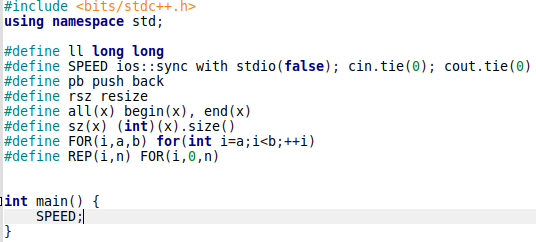
\includegraphics[scale=0.4]{template}

\section{Data Structures}
\subsection{Segment Tree}

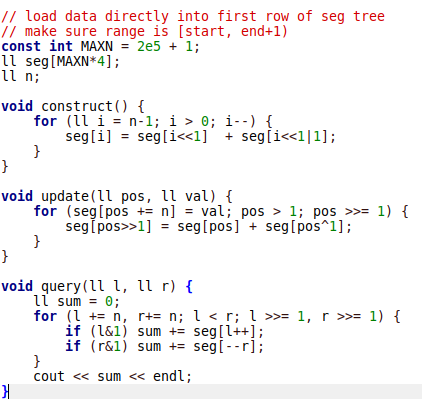
\includegraphics[scale=0.4]{segmenttree}

\subsection{Minimum Sparse}

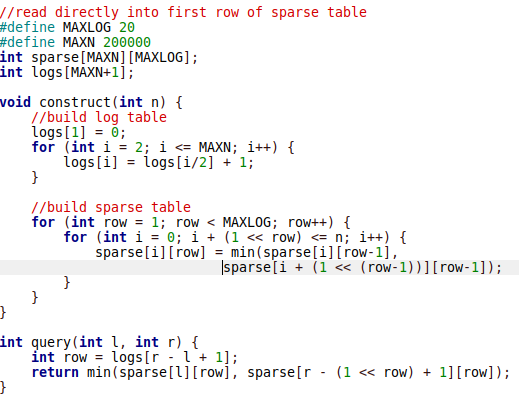
\includegraphics[scale=0.4]{sparsemin}

\subsection{Binary Jumping}

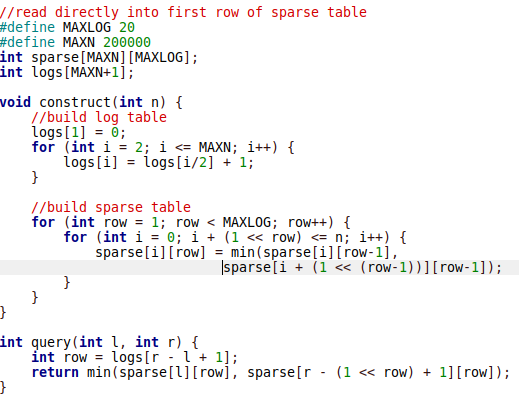
\includegraphics[scale=0.4]{sparsemin}

\section{Graph Algorithms}
\subsection{DFS with Cycle Detection}
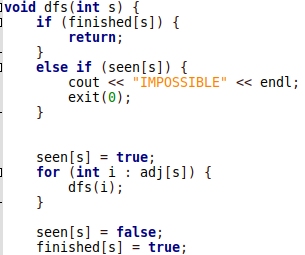
\includegraphics[scale=0.5]{dfs}
\subsection{BFS}
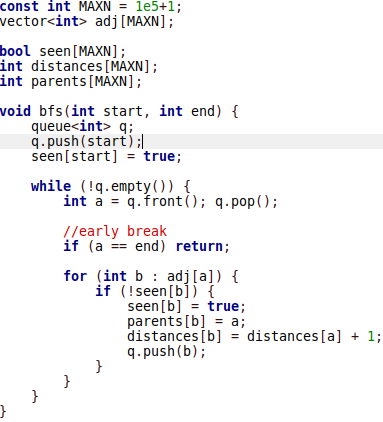
\includegraphics[scale=0.5]{bfs}
\subsection{BFS Route Reconstruction}
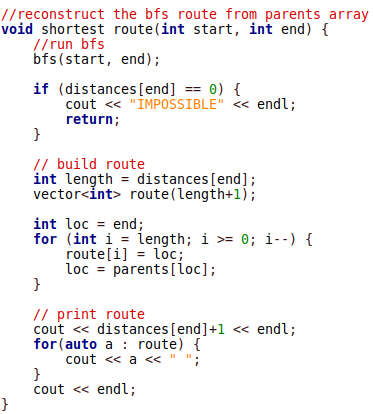
\includegraphics[scale=0.5]{bfsroutes}
\subsection{Djikstra}
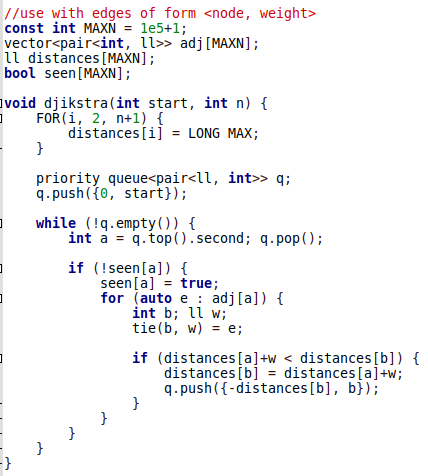
\includegraphics[scale=0.5]{djikstra}
\subsection{Bellman-Ford}

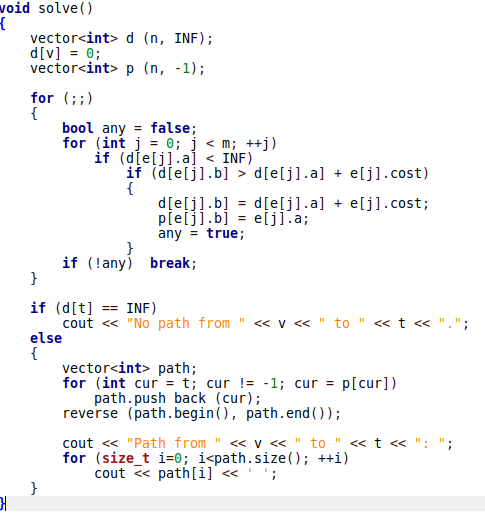
\includegraphics[scale=0.5]{bellmanford}

\subsection{Bellman-Ford with Negative Cycle Check}
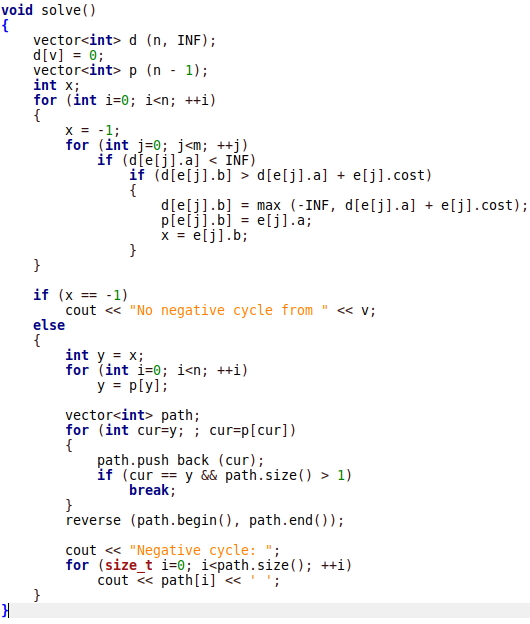
\includegraphics[scale=0.5]{bellmanfordneg}
\subsection{Floyd-Warshall}
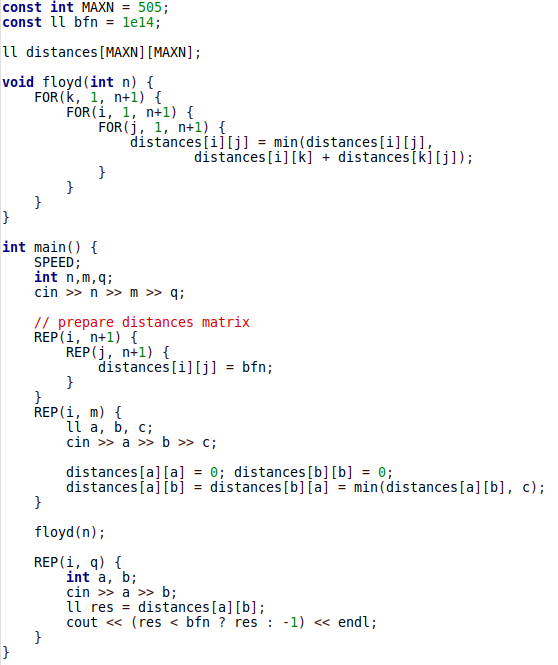
\includegraphics[scale=0.4]{floyd}
\subsection{Find Bridges of Graph}
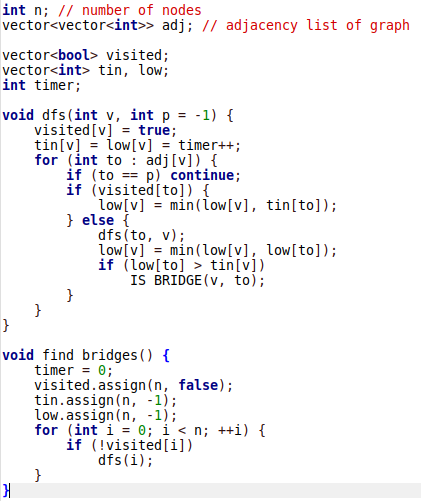
\includegraphics[scale=0.5]{bridges}
\subsection{Topological Sort}
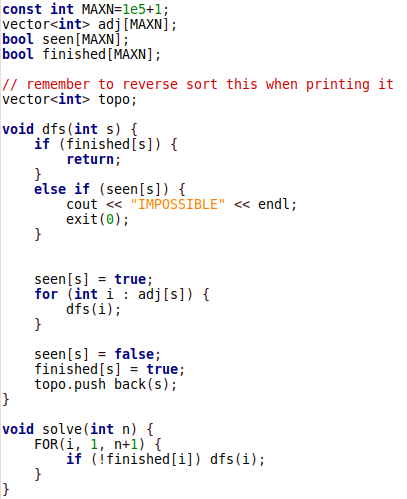
\includegraphics[scale=0.5]{topological}
\subsection{Kruskal with DSU}
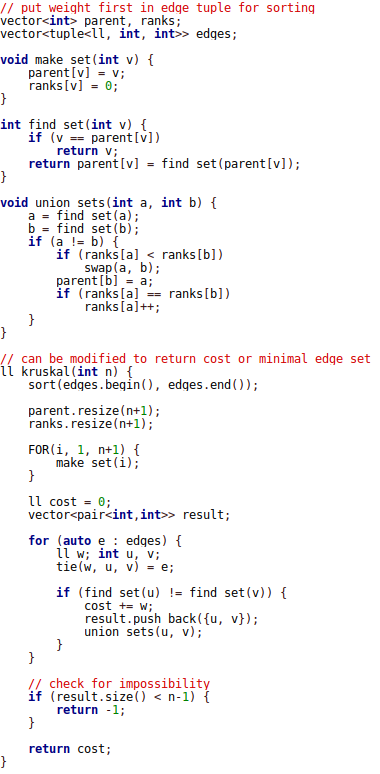
\includegraphics[scale=0.5]{kruskal}

\subsection{Connected Components}
For counting, use DFS and increment whenever the recursive call is completely finished. For listing, keep a vector that gets appended to during DFS. Print the vector, then reset it for the next component.

\subsection{Strongly Connected Components}

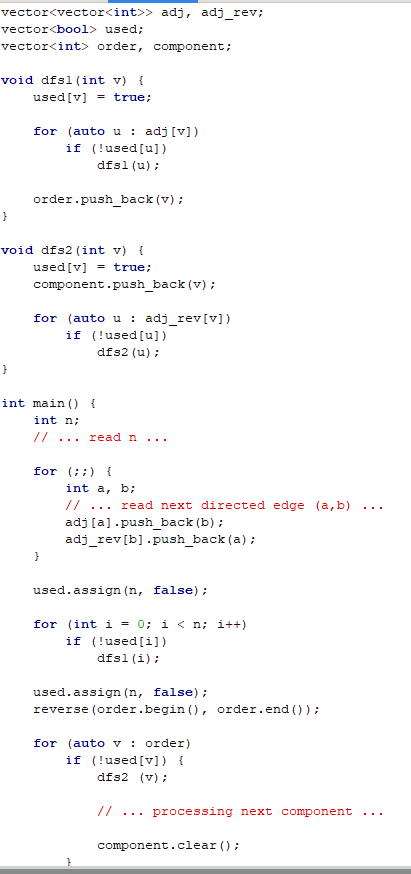
\includegraphics[scale=0.8]{kosaraju}

\subsection{Bipartite Check}


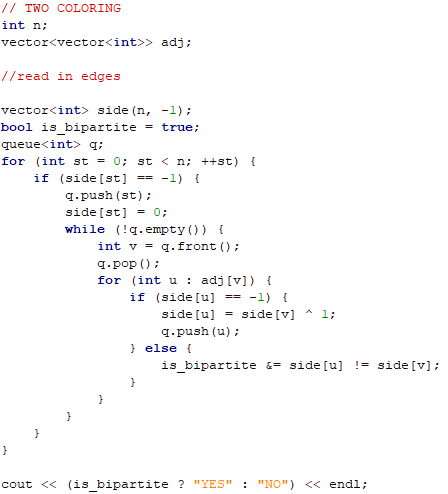
\includegraphics[scale=0.6]{twocoloring}

\subsection{Maximum Flow}

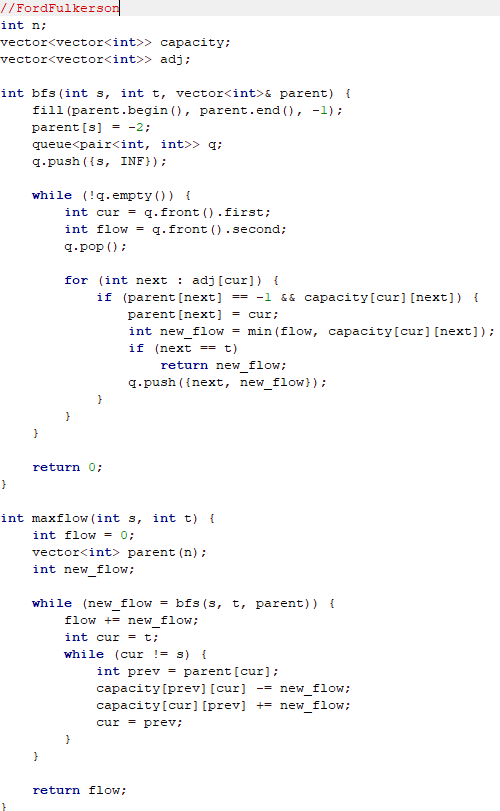
\includegraphics[scale=0.6]{fordfulkerson}

\subsection{Minimum Cost Flow}


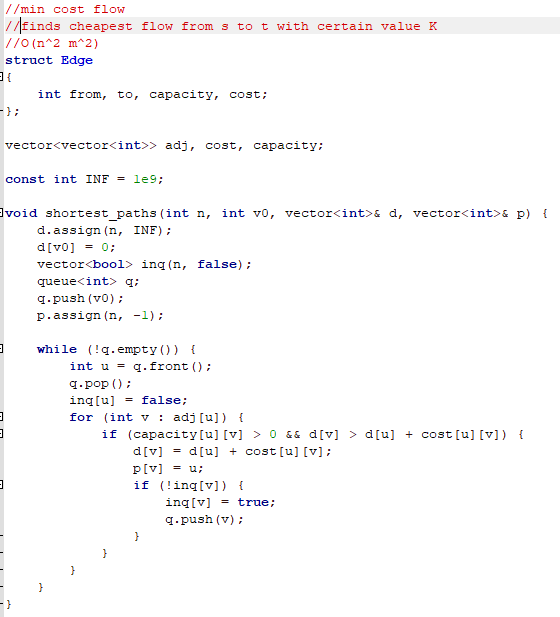
\includegraphics[scale=0.6]{mincostflowa}

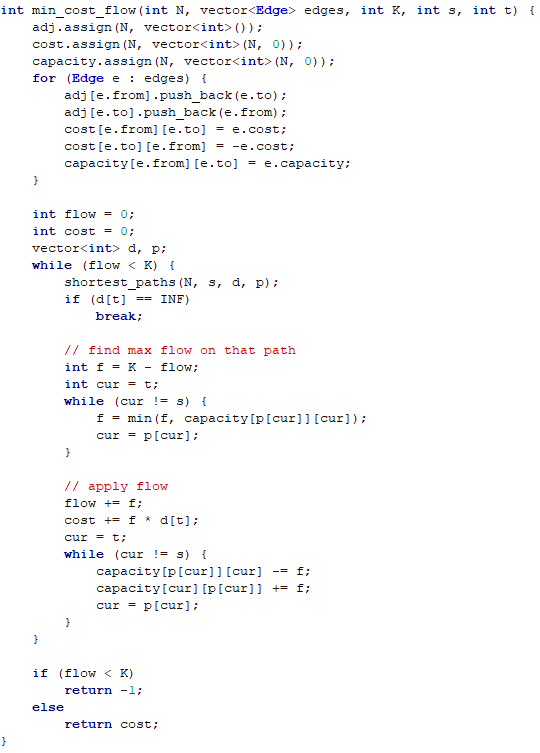
\includegraphics[scale=0.6]{mincostflowb}

\subsection{Bipartite Matching}


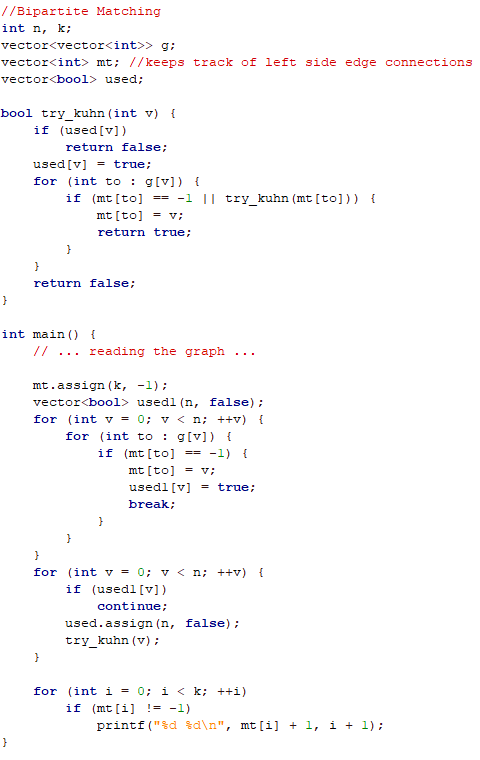
\includegraphics[scale=0.6]{bipartitematchign}

\subsection{Number of Paths of Fixed Length}
Suppose we have an adjacency matrix G, and we wish to find the number of paths with length k. G[i][j] is the number of edges from i to j. Raise the matrix G to the k-th power, then count the ones. Can use binary exponentiation if needed.
\subsection{2SAT}

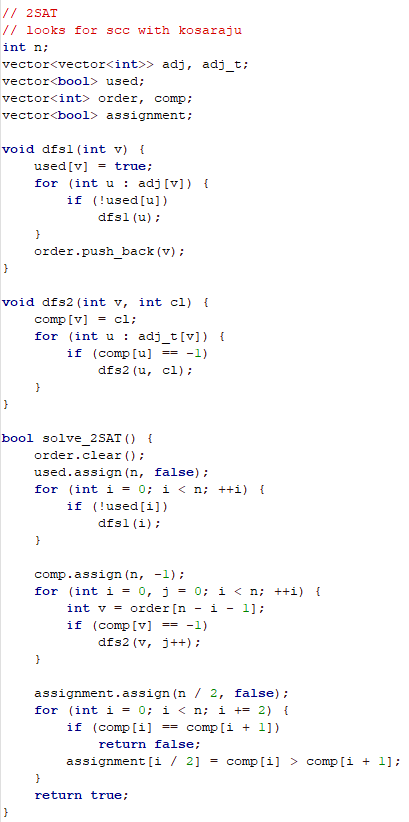
\includegraphics[scale=0.8]{2sata}

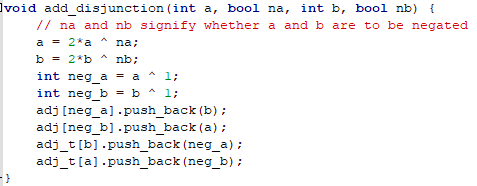
\includegraphics[scale=0.8]{2satb}
\subsection{TSP}

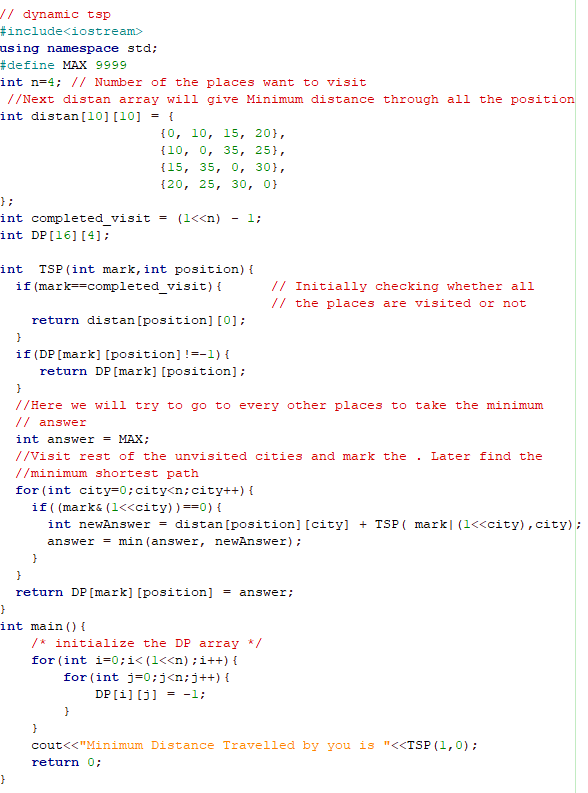
\includegraphics[scale=0.6]{tsp}

\subsection{Lowest Common Ancestor}


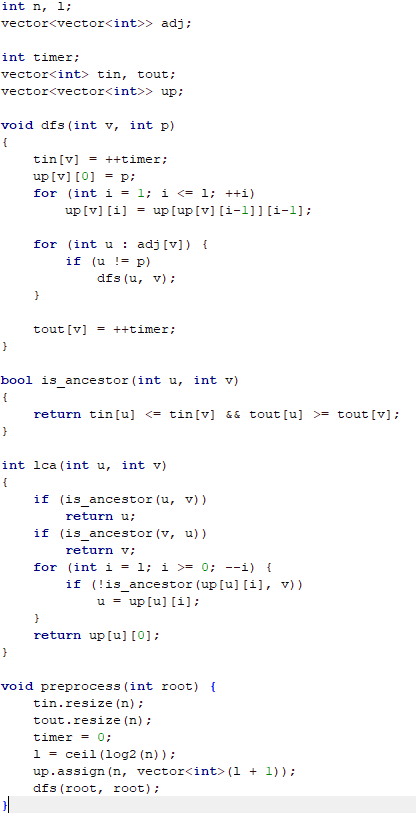
\includegraphics[scale=0.7]{lca}

\subsection{Eulerian Path}
Eulerian cycle only exists if degree of every node is even.
Eulerian path only exists if number of vertices with odd degree is 0 or 2.

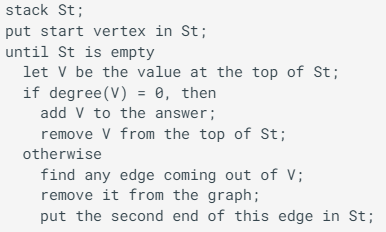
\includegraphics[scale=0.7]{eulerianpath}
    

\subsection{Hamiltonian Path}

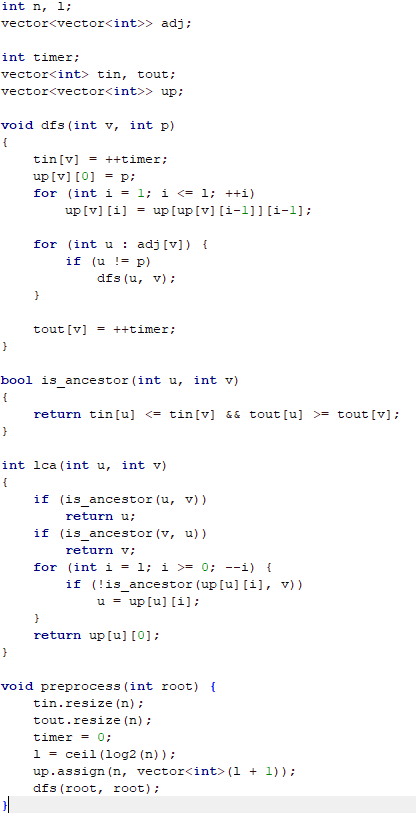
\includegraphics[scale=0.7]{lca}

\subsection{Centers}
Center of graph: set of vertices with minimum eccentricity. Use floyd warshall

Diameter of tree: BFS from v1. Last seen is v2. BFS from v2. Last seen is v3.

Center of tree: Do above and center is the middle of path from v2 to v3.

\section{Dynamic Programming}
\subsection{Longest Increasing Subseqeuence}

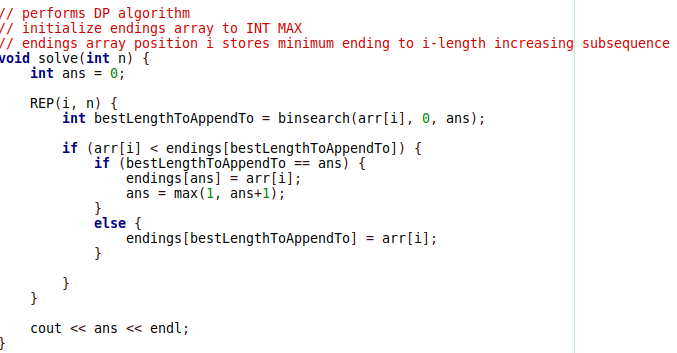
\includegraphics[scale=0.5]{lis}

\subsection{Longest Common Subsequence}

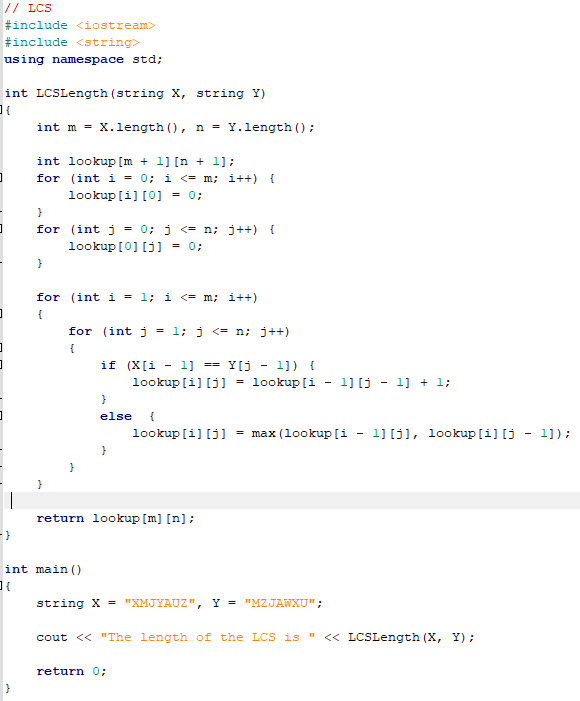
\includegraphics[scale=0.5]{lcs}

\subsection{Shortest Common Supersequence}

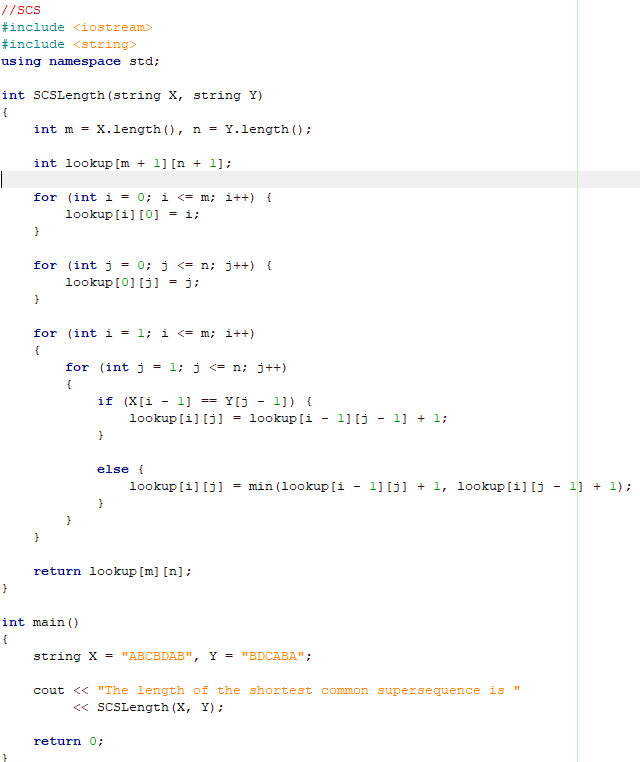
\includegraphics[scale=0.5]{scs}

\subsection{Edit Distance}

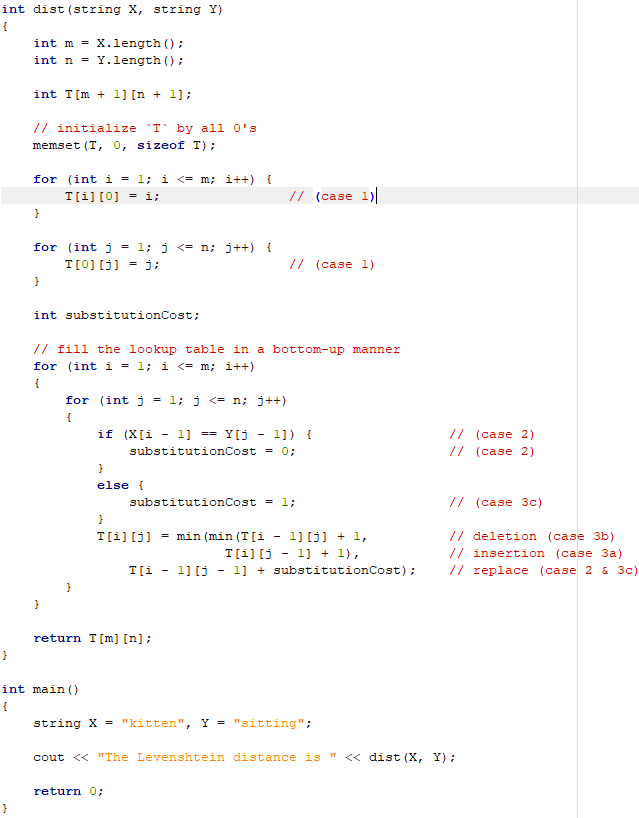
\includegraphics[scale=0.5]{edit}

\subsection{Coins Problem}
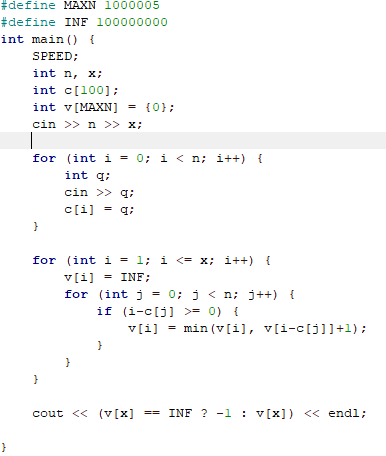
\includegraphics[scale=0.7]{coins}
\subsection{Knapsack}

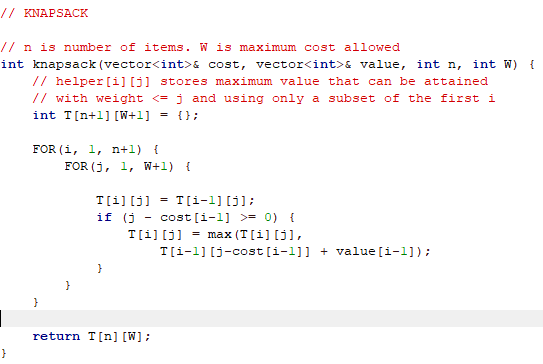
\includegraphics[scale=0.7]{knapsack}

\subsection{Partition}
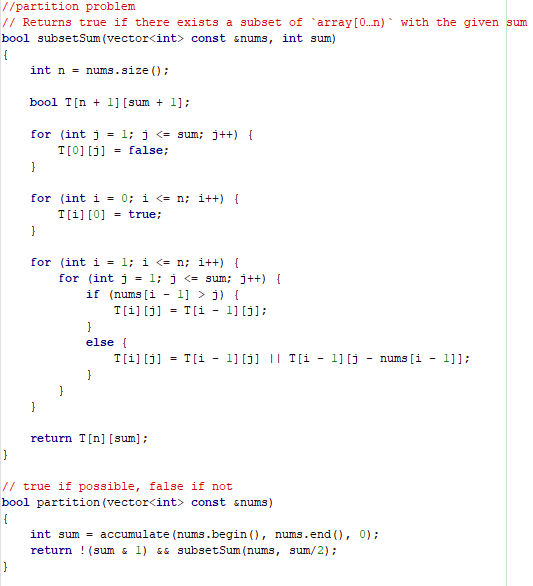
\includegraphics[scale=0.7]{partition}

\subsection{Rod Cutting}

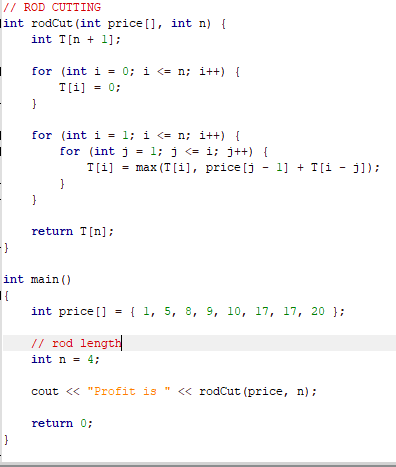
\includegraphics[scale=0.7]{rod}

\subsection{Word Break}

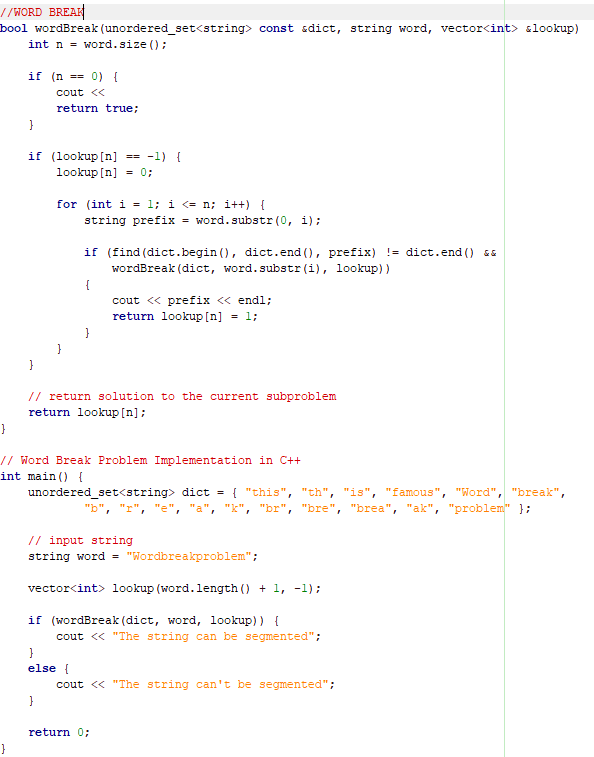
\includegraphics[scale=0.6]{wordbreak}

\subsection{Counting Tilings}
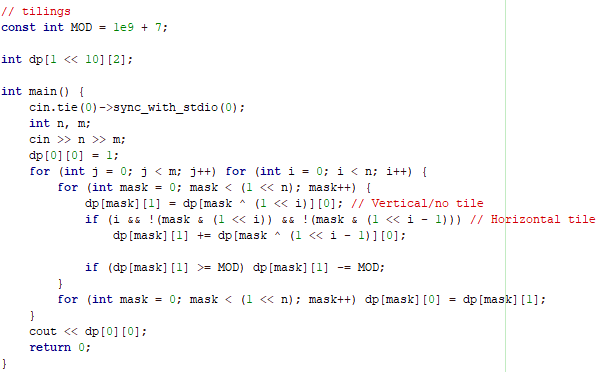
\includegraphics[scale=0.6]{tilings}
\section{Number Theoretic}
\subsection{Primality Testing}

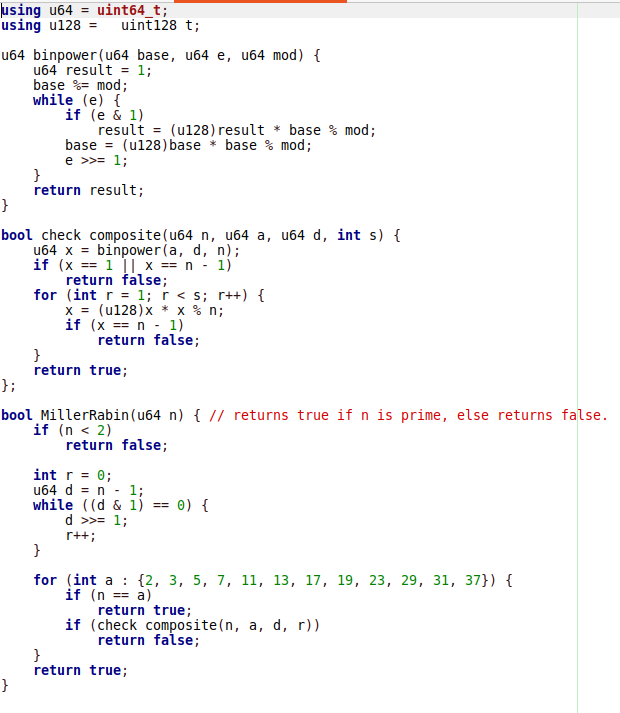
\includegraphics[scale=0.5]{millerrabin}

\subsection{Euler Totient}
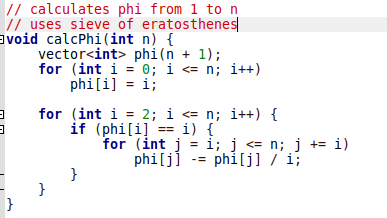
\includegraphics[scale=0.5]{eulertotient}

\subsection{Inclusion Exclusion}

\section{Strings}
\subsection{String Hashing}

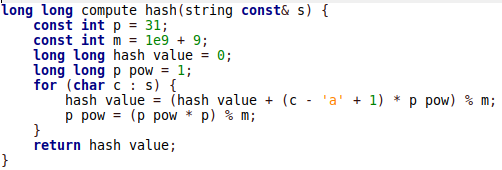
\includegraphics[scale=0.5]{hashing}

\subsection{Count unique strings in array}

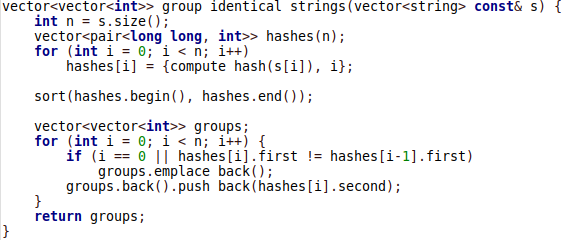
\includegraphics[scale=0.4]{identicalstrings}

\subsection{Count unique substrings of string}
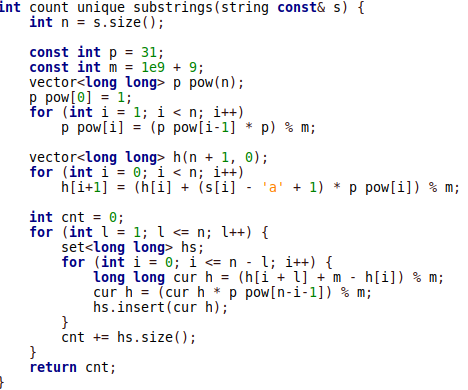
\includegraphics[scale=0.5]{uniquesubstrings}

\subsection{RabinKarp: String matching}
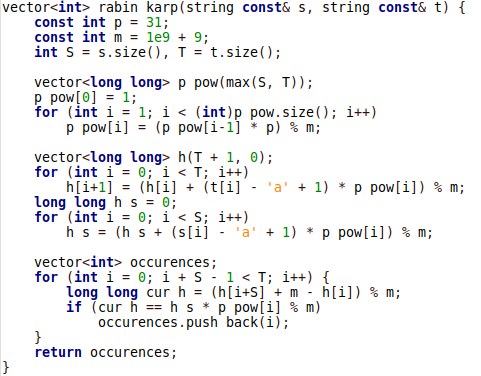
\includegraphics[scale=0.5]{rabinkarp}

\subsection{Knuth-Morris-Pratt}
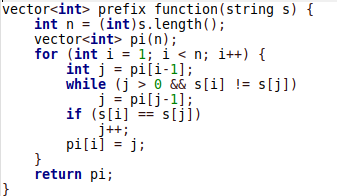
\includegraphics[scale=0.5]{kmp}

Uses:
1) Check if t is in s. Run KMP with the string s+\#+t.

\subsection{Manacher Palindromes}
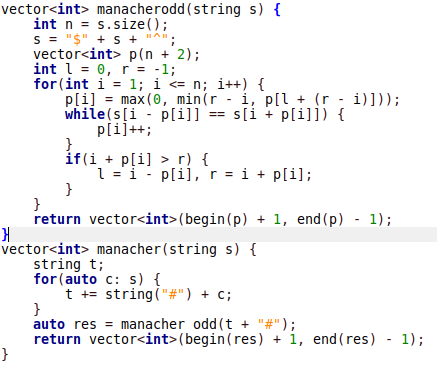
\includegraphics[scale=0.5]{manacher}


\section{Miscellaneous}
\subsection{Binary Search}

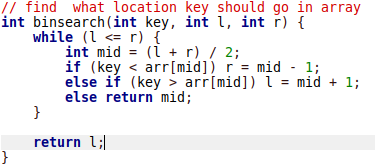
\includegraphics[scale=0.5]{binsearch}

\subsection{Binary Exponentiation}

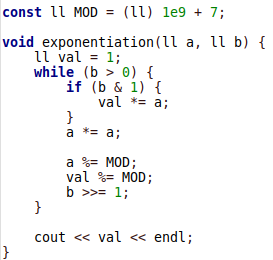
\includegraphics[scale=0.5]{binexp}

\subsection{Gray Code}

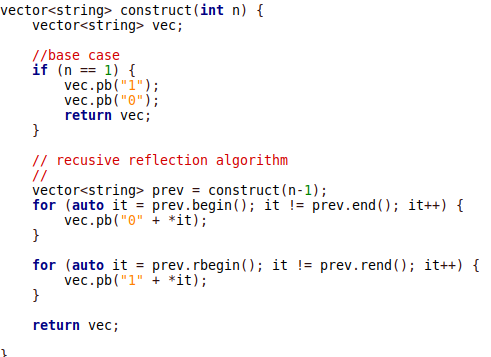
\includegraphics[scale=0.5]{graycode}

\subsection{Towers of Hanoi}
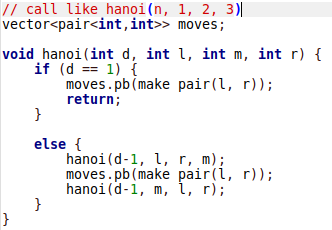
\includegraphics[scale=0.5]{hanoi}

\subsection{Expression Parsing}

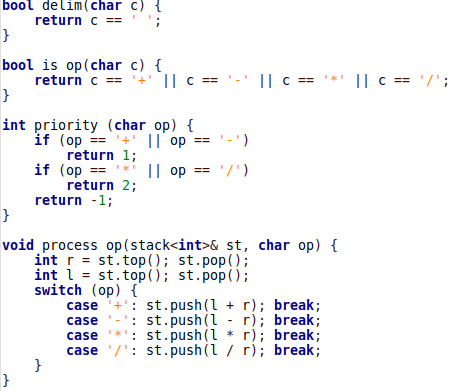
\includegraphics[scale=0.5]{parsea}

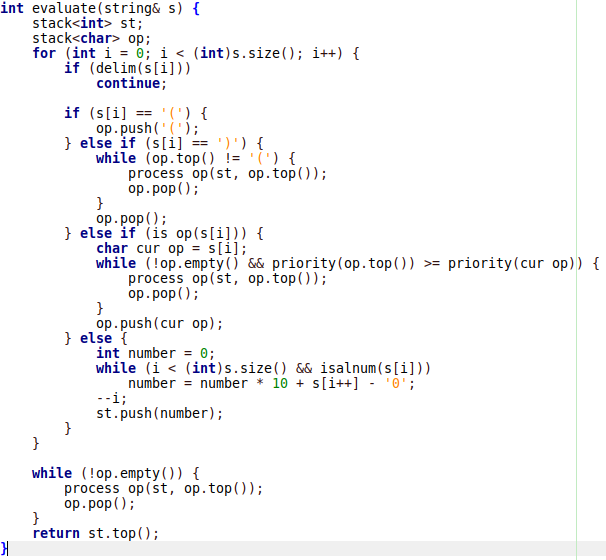
\includegraphics[scale=0.4]{parseb}

\subsection{Balanced Sequences}


\includegraphics[scale=0.6]{balanced}


\subsection{Korder Statistic}
C++ standard library has this implemented already. The function is called $nth\_element$.

\includegraphics[scale=0.4]{nthelement}

\subsection{Josephus Queries}

\includegraphics[scale=0.5]{josephus}

\subsection{Convex Hull}

\includegraphics[scale=0.6]{convex}
\end{document}
